\subsection{Discusión teórica de las desviaciones del modelo}

El modelo del rotor rígido constituye una excelente primera aproximación para describir la rotación de moléculas diatómicas, pero en la práctica se observan pequeñas desviaciones respecto a las predicciones ideales. Estas discrepancias se deben principalmente a tres factores: la no-rigidez molecular, el acoplamiento con vibraciones internas y la sustitución isotópica.

\subsubsection*{Rotor no rígido y corrección centrífuga}

Durante la rotación molecular, las fuerzas centrífugas tienden a estirar el enlace, aumentando ligeramente la distancia internuclear efectiva \( r \). Este efecto reduce la constante rotacional \( B \) con el aumento de \( J \), ya que \( B \propto 1/I \propto 1/r^2 \). Para tener en cuenta esta variación se introduce el término de corrección centrífuga \( D \), de modo que los niveles de energía rotacional se expresan como:
\[
E_J = B J (J + 1) - D [J (J + 1)]^2,
\]
donde \( D \ll B \) y su valor típico se obtiene experimentalmente del ajuste espectral. En el caso del HCl, \( D \approx 5.3 \times 10^{-4}~\text{cm}^{-1} \), lo que implica un corrimiento de las líneas hacia frecuencias ligeramente menores conforme aumenta \( J \).

\begin{figure}[H]
\centering
\begin{tikzpicture}[xscale=1.2,yscale=1]
  \draw[->] (0,0) -- (8,0) node[right]{Frecuencia (GHz)};
  \draw[->] (0,0) -- (0,3) node[above]{Intensidad (a.u.)};

  \foreach \x in {1,...,6}{
    \draw[thick,blue!70] (1.0*\x,0) -- (1.0*\x,1.5);
  }
  \foreach \x in {1,...,6}{
    \draw[thick,red!60,dashed] (0.98*\x,0) -- (0.98*\x,1.2);
  }

  \node[blue!70] at (7,2.5){\small Modelo rígido};
  \node[red!60] at (7,2.1){\small Rotor no rígido};
\end{tikzpicture}
\caption{Comparación entre el espectro del rotor rígido (líneas azules) y el no rígido (rojas discontinuas). La corrección centrífuga desplaza las líneas hacia frecuencias ligeramente menores.}
\end{figure}

\subsubsection*{Efecto isotópico}

La constante rotacional depende inversamente del momento de inercia \( I = \mu r^2 \). Por tanto, al sustituir un isótopo, cambia la masa reducida \(\mu\) y, con ello, el espaciado entre líneas. En el caso del HCl, la sustitución de \(^{35}\text{Cl}\) por \(^{37}\text{Cl}\) modifica \(\mu\) en aproximadamente un 5\%, produciendo una disminución correspondiente en la constante \(B\):
\[
\frac{B(^{37}\text{Cl})}{B(^{35}\text{Cl})} = \frac{\mu(^{35}\text{Cl})}{\mu(^{37}\text{Cl})} \approx 0.95.
\]
Esto da lugar a dos conjuntos de líneas muy próximas entre sí, observadas experimentalmente como un \textbf{doblete isotópico}, lo que permite determinar con precisión las masas relativas de los átomos constituyentes.

\begin{figure}[H]
\centering
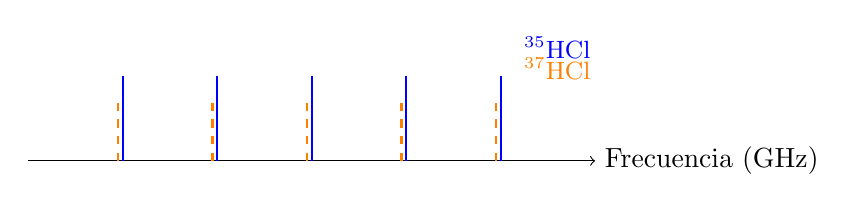
\begin{tikzpicture}[xscale=1.2,yscale=0.9]
  \draw[->] (0,0) -- (6,0) node[right]{Frecuencia (GHz)};
  \foreach \x in {1,...,5}{
    \draw[thick,blue] (\x,0) -- (\x,1.2);
    \draw[thick,orange,dashed] (\x-0.05,0) -- (\x-0.05,0.9);
  }
  \node[blue] at (5.6,1.6){\small $^{35}$HCl};
  \node[orange] at (5.6,1.3){\small $^{37}$HCl};
\end{tikzpicture}
\caption{Efecto isotópico en el espectro del HCl: la sustitución de $^{35}$Cl por $^{37}$Cl genera un doblete debido al cambio en la masa reducida.}
\end{figure}

\subsubsection*{Interacción vibración-rotación}

En un tratamiento más refinado, el movimiento rotacional no está completamente desacoplado de las vibraciones moleculares. Al excitarse un modo vibracional, cambia la distancia media internuclear, y con ello el momento de inercia. Por tanto, la constante rotacional en el nivel vibracional \(v\) se expresa como:
\[
B_v = B_e - \alpha_e \left(v + \frac{1}{2}\right),
\]
donde \(B_e\) es la constante rotacional en el equilibrio y \(\alpha_e\) representa la constante de acoplamiento vibración-rotación. Este término explica la ligera disminución de \(B\) observada con el aumento de energía vibracional.

\subsubsection*{Síntesis de los efectos}

La combinación de los tres factores anteriores —no-rigidez, acoplamiento vibracional y sustitución isotópica— explica las pequeñas desviaciones observadas en los espectros experimentales respecto al modelo ideal. La espectroscopía de microondas, con su altísima resolución, permite cuantificar dichas correcciones y extraer información de precisión sobre la estructura interna de las moléculas.

En conjunto, estas correcciones no invalidan el modelo del rotor rígido, sino que lo \textbf{enriquecen}, permitiendo un ajuste más fiel a los datos experimentales y proporcionando una conexión directa entre la teoría cuántica y la observación espectral.

